\section[L'indexation dans AGORHA]{L'indexation à l'aide du thésaurus Garnier dans les bases de données d'AGORHA}

Ces graphiques sont disponibles au lien suivant : \url{https://public.tableau.com/app/profile/pierre.husson/viz/AGORHA/UtilisationdeGarnierdansAgorha}


\begin{figure}[H]
    \centering
    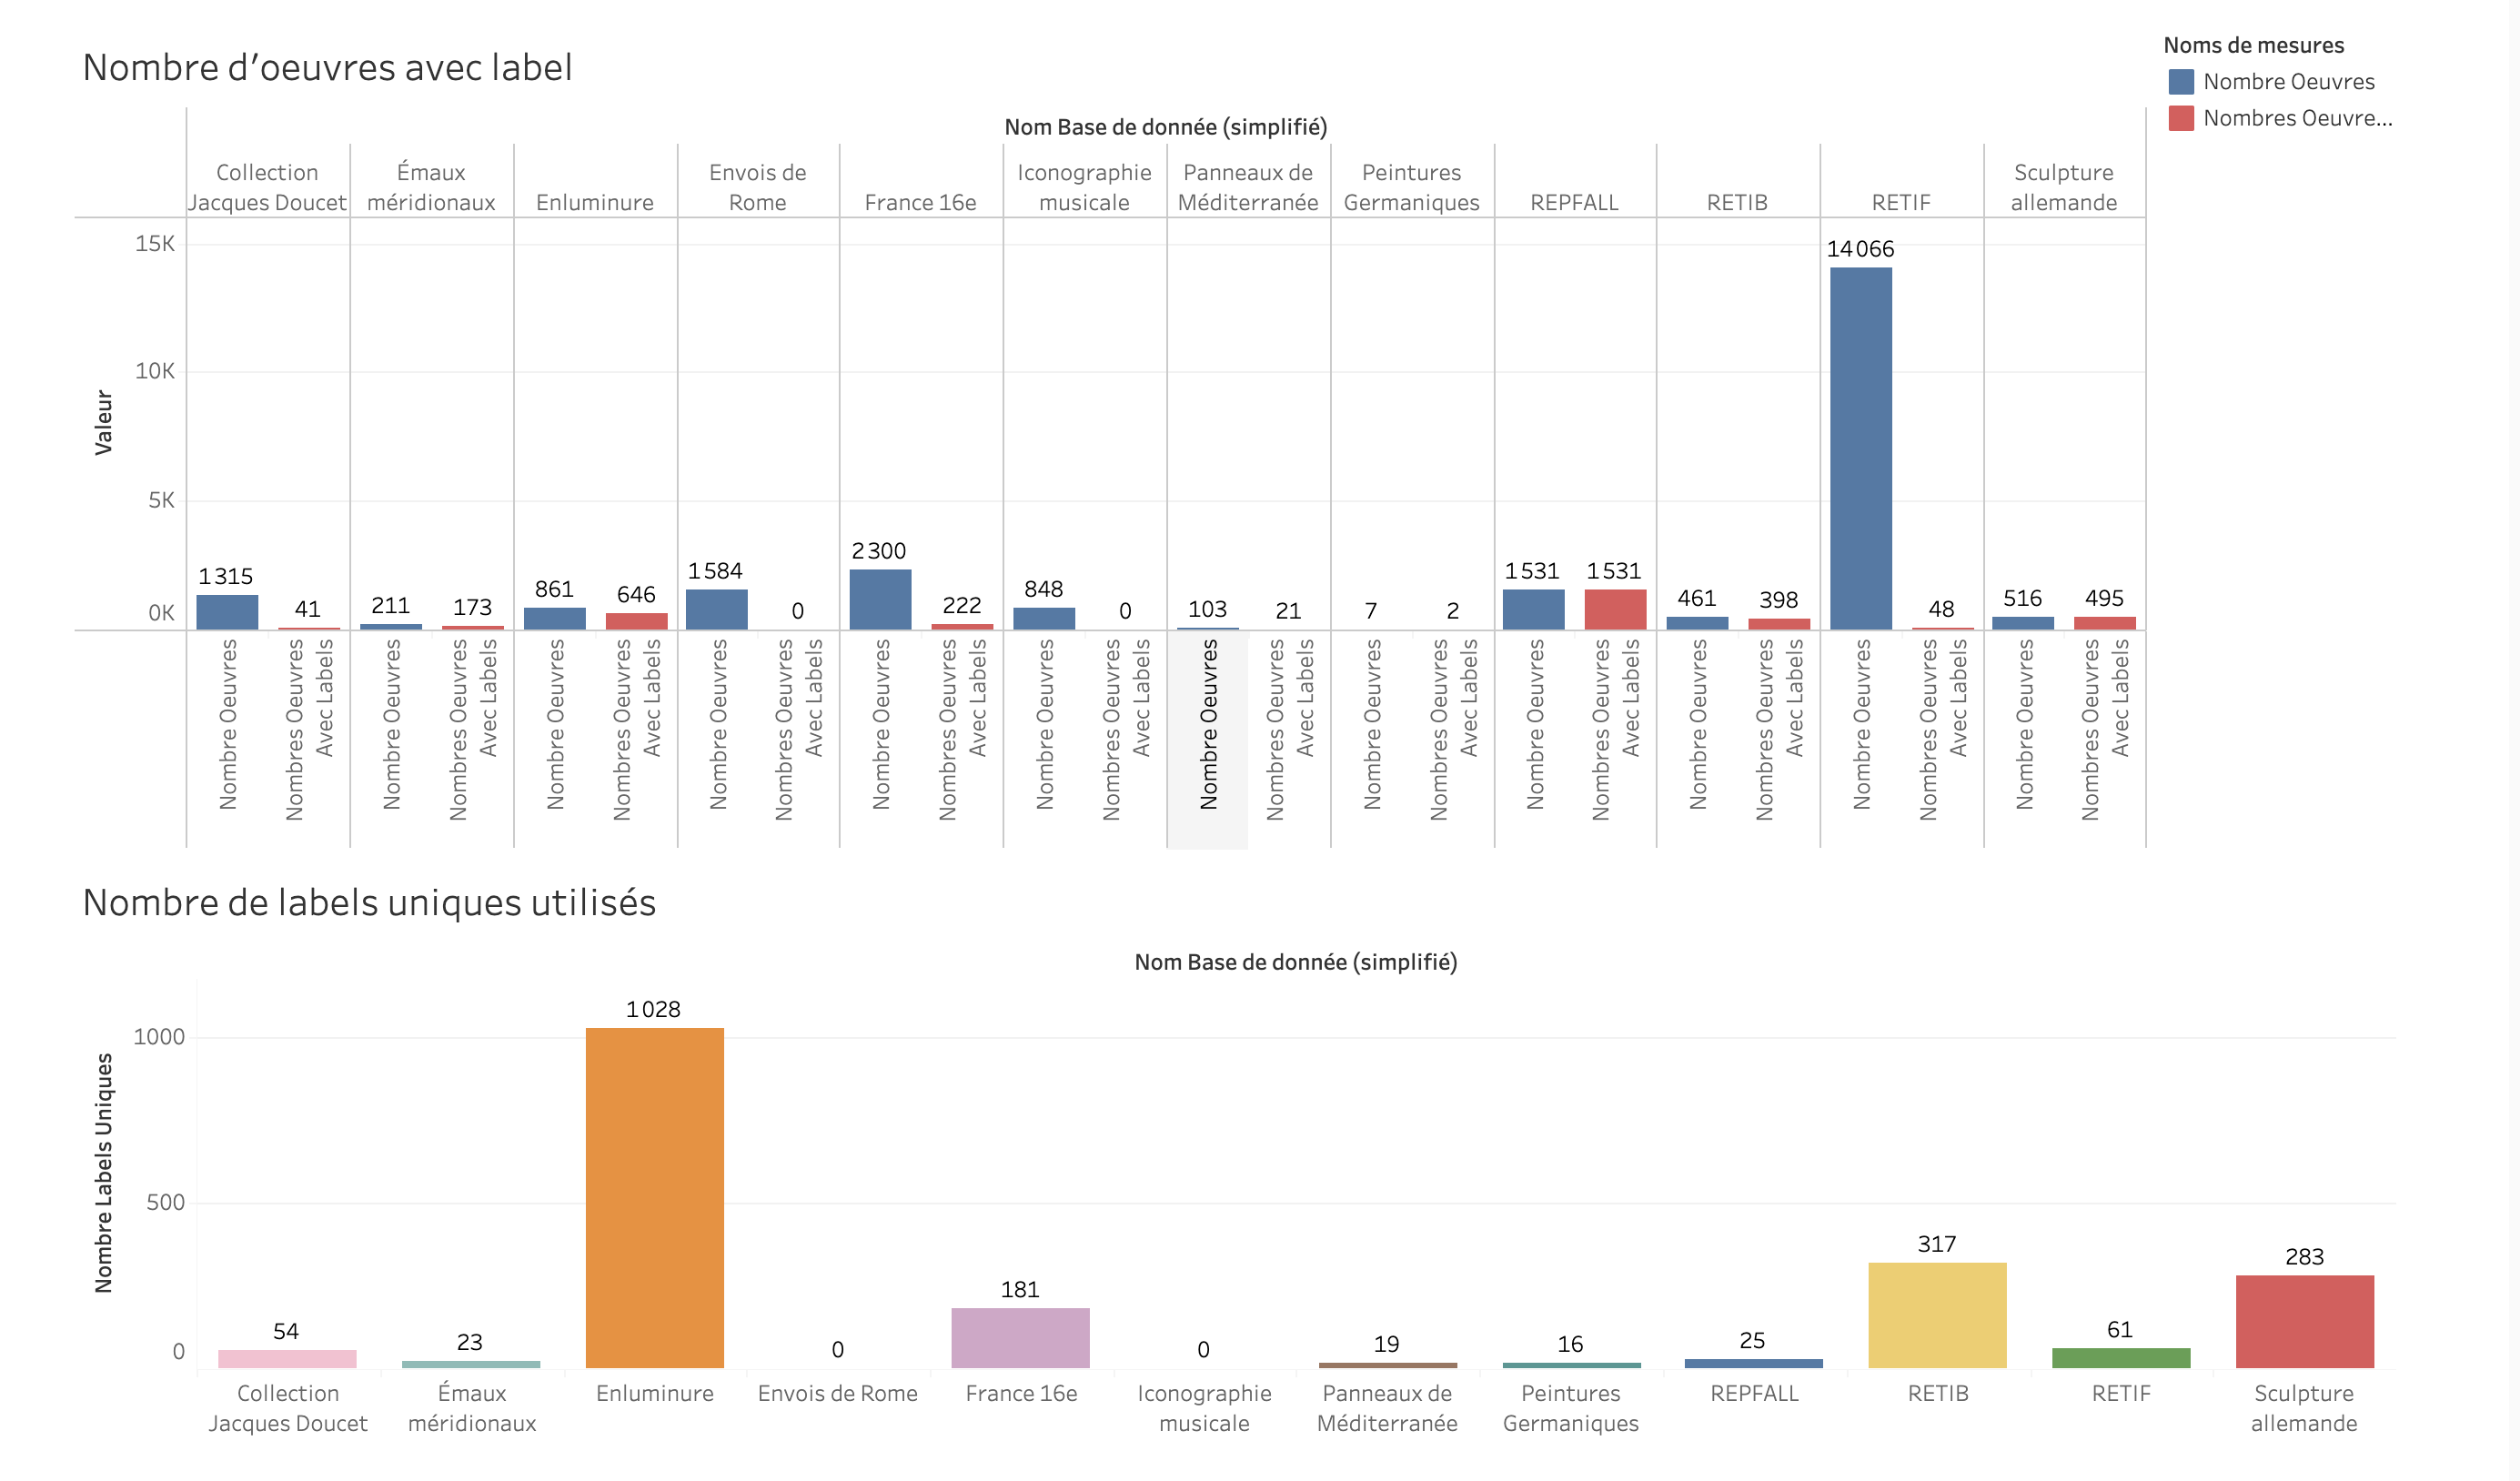
\includegraphics[height=0.4\textheight]{annexes/stats/graphiqueGarnier1A.png}
    \caption{Graphiques montrant le nombre de notices indexées avec au moins un label dans 12 bases d'AGORHA, et le nombre de labels distincts utilisés par bases.}
    \label{stat:Garnier1A}
\end{figure}


\begin{figure}[H]
    \centering
    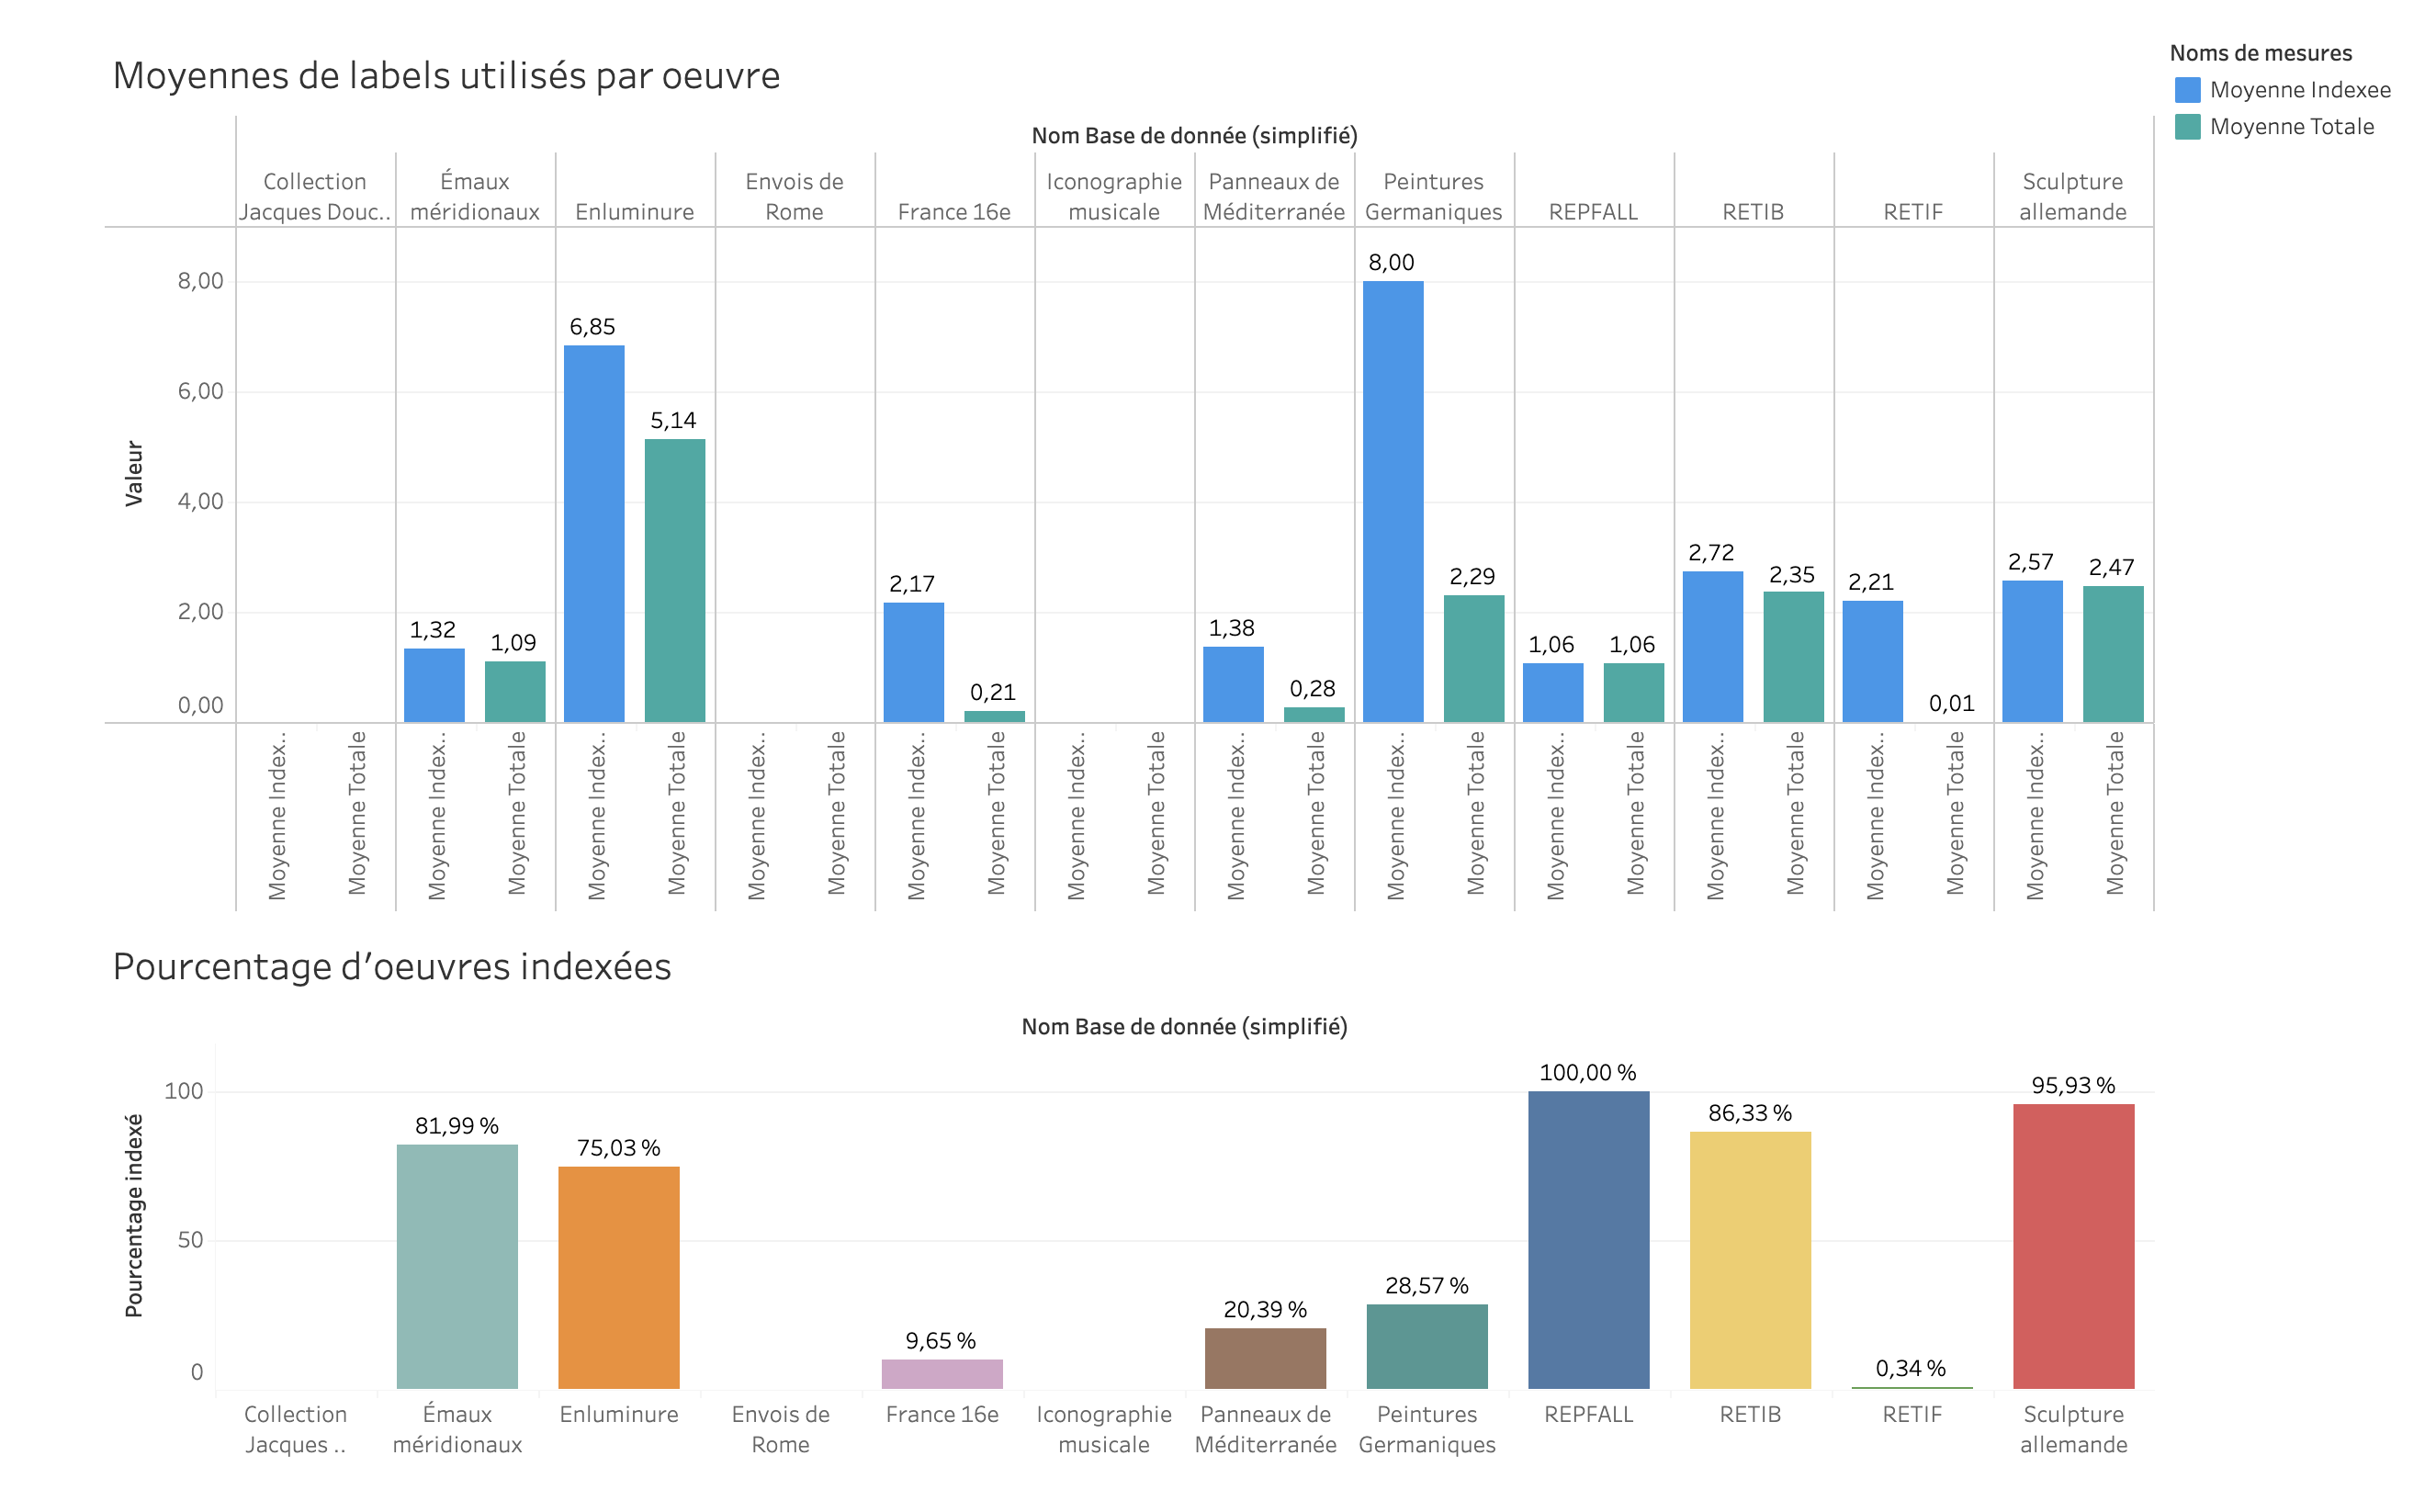
\includegraphics[height=0.4\textheight]{annexes/stats/graphiqueGarnier1B.png}
    \caption{Graphique montrant la moyenne de labels utilisés par notices dans 12 bases d'AGORHA, pour les oeuvres indexées et toutes les oeuvres ; et le pourcentage de d'oeuvres qui possèdent au moins un label par base de données.}
    \label{stat:Garnier1B}
\end{figure}


\section{Code Python pour structurer le thésaurus Garnier en json}
\label{pythonGarnier}

\begin{minted}[frame=lines, linenos, fontsize=\small]{python}
import json
from rdflib import Graph, Namespace
from collections import defaultdict

"""
Ce script génère deux fichiers pour faciliter l’exploitation du thésaurus Garnier de l’INHA à partir d’un fichier XML-RDF :
- un fichier JSON qui représente la hiérarchie complète des concepts et qui inclut, pour chacun d'entre eux : l’URI (id), le label préféré (prefLabel), les labels alternatifs (altLabels), les concepts enfants (children). La hiérarchie est structurée sous forme de dictionnaires imbriqués, et tous les concepts sont triés par ordre alphabétique.

- un fichier TXT qui contient uniquement les labels principaux (prefLabel) des concepts. La hiérarchie est reproduite grâce à une indentation par niveau.
"""

rdf_entree = "thesaurusGarnierINHA.rdf"
resultat_json = "JSONthesaurusGarnierINHA.json"
resultat_txt = "TXTthesaurusGarnierINHA.txt"

# Charger le fichier XML-RDF
g = Graph()
g.parse(rdf_entree, format="xml")

# définition du namespace SKOS
SKOS = Namespace("http://www.w3.org/2004/02/skos/core#")

# préparation des dictionnaires
labels = {}
alt_labels = defaultdict(list)
broader_relations = defaultdict(list)

# Extraction des "prefLabel"
for s, p, o in g.triples((None, SKOS.prefLabel, None)):
    labels[str(s)] = str(o)

# Extraction des "altLabel"
for s, p, o in g.triples((None, SKOS.altLabel, None)):
    alt_labels[str(s)].append(str(o))

# identification de la hierarchie parents enfants des concepts
for s, p, o in g.triples((None, SKOS.broader, None)):
    broader_relations[str(o)].append(str(s))

# Trouver les concepts racines (càd les concepts sans skos:broader)
all_concepts = set(labels.keys()) | set(alt_labels.keys())
children = set()
for children_list in broader_relations.values():
    children.update(children_list)

roots = list(all_concepts - children)

# fonction récursive pour créer la hiérarchie JSON
def build_hierarchy(concept_uri):
    children_sorted = sorted(
        broader_relations.get(concept_uri, []),
        key=lambda x: labels.get(x, "").lower()
    )
    return {
        "id": concept_uri,
        "label": labels.get(concept_uri, ""),
        "altLabels": sorted(alt_labels.get(concept_uri, []), key=str.lower),
        "children": [build_hierarchy(child) for child in children_sorted]
    }

# Créer la hiérarchie complète (racines triées dans l'ordre alphabétique des labels)
roots_sorted = sorted(roots, key=lambda x: labels.get(x, "").lower())
hierarchy = [build_hierarchy(root) for root in roots_sorted]

# Sauvegarder en JSON
with open(resultat_json, "w", encoding="utf-8") as f:
    json.dump(hierarchy, f, ensure_ascii=False, indent=2)
print(f"{resultat_json} a bien été créé !")

# Sauvegarde d'un txt indenté contenant seulement les labels
def write_txt(node, f, indent=0):
    f.write("\t" * indent + str(node["label"]) + "\n")
    for child in node["children"]:
        write_txt(child, f, indent + 1)

with open(resultat_txt, "w", encoding="utf-8") as f:
    for root in hierarchy:
        write_txt(root, f)
print(f"{resultat_txt} a bien été créé !")
\end{minted}
